Nick Vosseteig

2014-11-21

building, wiring, programming

\begin{tabular}{|p{5cm}|p{5cm}|}
 \hline
 building&
We moved back the large spinner and added a new intake device so we can pick up balls from the walls.
 \\
 \hline
wiring&
Alex, David, and I worked on the wiring after finding a few problems. David created a wiring diagram.
 \\
 \hline
programming&
I updated the program so that it works with the new configuration
 \\
 \hline
\end{tabular}

\section*{building}
After adding the larger spinner, we realized that, while it does work better, it has the disadvantage of not being able to pick up balls that are shoved against the wall. We added a smaller spinner on the front to get the balls off the wall and moved the larger spinner further back on the robot. We also created a prototype ramp out of cardboard that worked much better than the makeshift ramp we were using to test before.
\section*{Wiring}
We found a few problems with the wiring and got them fixed.

Here is a picture of the new setup with both spinners and the wiring on the sides:
\begin{center}
 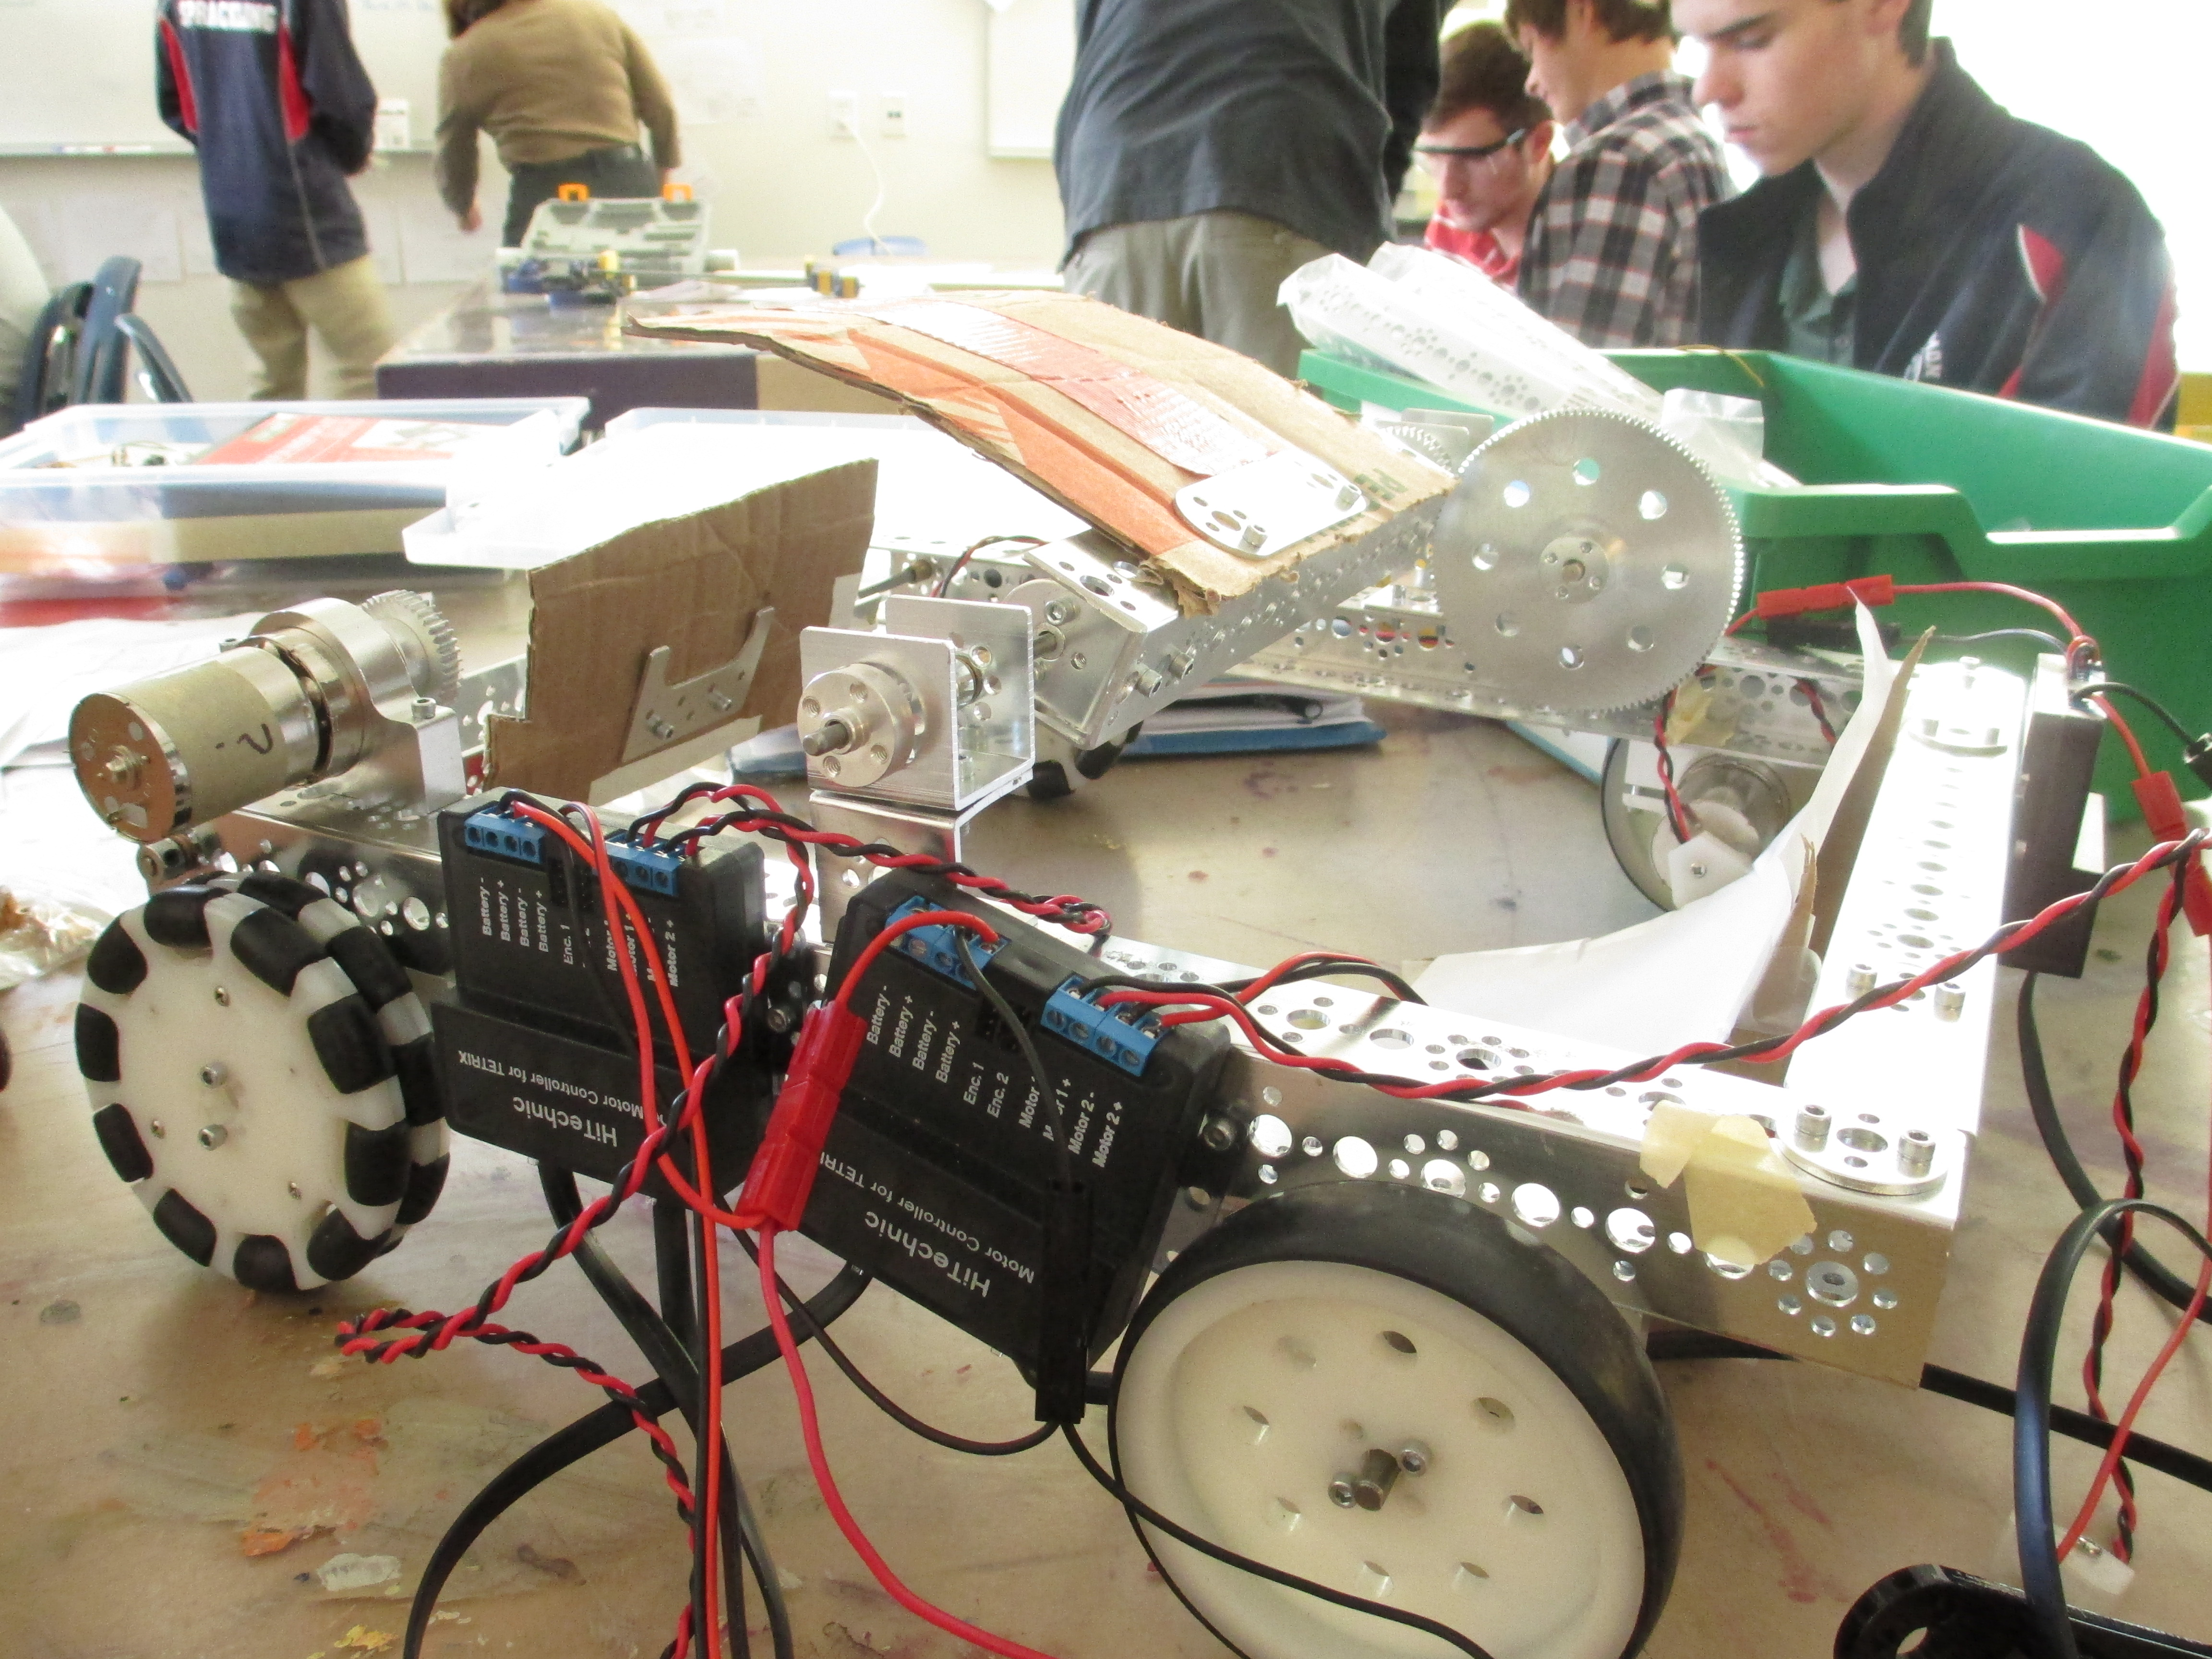
\includegraphics[width=215px]{./Entries/Images/RobotDesignForNovemberTwentyFirstTwoThousandAndFourteenWithIntakeLauncherAndRampWiringIncludedILoveAlexHeIsTheBestNic.JPG}
\end{center}